\section{Introduction}

When software vulnerabilities such as Heartbleed or Log4Shell are disclosed, they receive a CVE identifier and a short text description, but the description alone does not tell a security team how urgently to act.
Teams therefore rely on structured \emph{enrichment} consisting of a CVSS v3.1 vector that records how the flaw is exploited and what it affects, the base score (0--10) and severity tier that follow from that vector, and a CWE category for the type of weakness~\citep{first2019cvss31}.
Scanners, patch managers, and incident responders sort their work queues by these fields, so a CVE that lacks them gives defenders little basis for deciding what to fix first.

For most CVEs, this enrichment was supplied by the National Vulnerability Database (NVD) at NIST, which has not kept pace with the volume of disclosures.
A backlog formed in early 2024, and on 15 April 2026 NIST announced that it would enrich only CVEs in CISA's Known Exploited Vulnerabilities catalog, CVEs in software used by the federal government, and critical software under Executive Order 14028, with every other CVE marked ``Lowest Priority -- not scheduled for immediate enrichment''~\citep{nist2026nvd}.
For most new CVEs, defenders therefore receive only the description and whatever score the reporting organization chose to supply.

The task studied here, referred to as \textbf{CVE enrichment}, is to predict from the description alone the eight CVSS v3.1 vector components, the base score, the severity tier, and the CWE (Figure~\ref{fig:task}), using only public data and comparing TF-IDF classifiers, a small instruction-tuned language model used zero-shot, and the same model fine-tuned with LoRA.

\begin{figure}[t]
\centering
\begin{tikzpicture}[
  box/.style={draw=black!45, rounded corners=2pt, align=left, font=\footnotesize, inner sep=5pt},
  arr/.style={-{Stealth[length=5pt]}, black!60, thick}]
\node[box, text width=4.3cm] (desc) {\textbf{Description} (CVE-2024-0003)\\[2pt]
``A condition exists in FlashArray Purity whereby a malicious user could use a remote administrative service to create an account on the array allowing privileged access.''};
\node[box, right=1.1cm of desc, text width=3.5cm] (vec) {\textbf{CVSS v3.1 vector}\\[2pt]
\texttt{AV:N/AC:L/PR:H/UI:N}\\ \texttt{S:U/C:H/I:H/A:H}\\[3pt]
\textbf{CWE}: CWE-269};
\node[box, right=1.1cm of vec, text width=2.1cm] (score) {\textbf{Computed}\\[2pt]
Score: 7.2\\ Severity: \textsc{High}};
\draw[arr] (desc) -- node[above, font=\scriptsize, inner sep=2pt]{model} (vec);
\draw[arr] (vec) -- node[above, font=\scriptsize, inner sep=2pt]{formula} (score);
\end{tikzpicture}
\caption{CVE enrichment for CVE-2024-0003. A model reads the description and predicts the eight CVSS components and the CWE, and in the formula variant the score and severity are computed from the predicted vector with the CVSS v3.1 equations so that the three always agree.}
\label{fig:task}
\end{figure}

The data are split by time, with training on CVEs from 2022--2023 and testing on every usable CVE from 2024, so that no model is scored on a period it has already seen.
This design avoids the leakage that random splits introduce when near-duplicate descriptions from the same product and month fall on both sides of the split, as they can in several public models.
Because the CVSS base score and severity are fixed functions of the eight vector components, the components are predicted and the score is computed with the CVSS formula, following \citet{elbaz2020fighting} and \citet{shahid2021cvssbert}.
The comparison then measures both what this computation adds over predicting the score directly and whether a language model's own score agrees with the vector it writes.

On all \nTest{} test CVEs, the fine-tuned model is the strongest system on every field (Figure~\ref{fig:headline}), reaching \nLoRAfSev\% severity accuracy and \nLoRAfCwe\% CWE accuracy and predicting the exact CVSS vector for \nLoRAfVec\% of CVEs, \nDiffLRfSev{} to \nDiffLRfVec{} points ahead of TF-IDF logistic regression.
After \nLoraTrainHours{} hours of fine-tuning, its scores agree with its own vectors on \nLoRAScoreCons\% of CVEs, compared with only \nZSScoreCons\% for the same model used zero-shot.

\begin{figure}[t]
\centering
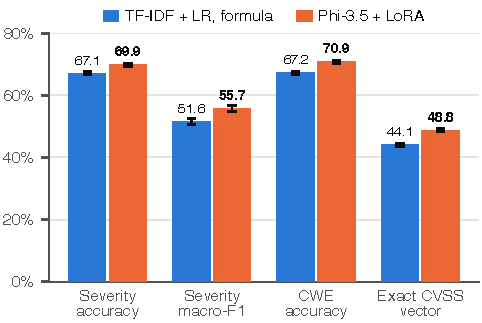
\includegraphics[width=0.68\linewidth]{figures/fig_headline.pdf}
\caption{Severity accuracy, severity macro-F1, CWE accuracy, and exact-vector rate for fine-tuned Phi-3.5 and TF-IDF logistic regression with formula scoring on the full 2024 test set (\nTest{} CVEs), with 95\% bootstrap intervals as error bars.}
\label{fig:headline}
\end{figure}
